\documentclass[t,usenames,dvipsnames]{beamer}
\usetheme{Copenhagen}
\setbeamertemplate{headline}{} % remove toc from headers
\beamertemplatenavigationsymbolsempty

\usepackage{amsmath, tikz, xcolor}
\usetikzlibrary{arrows.meta}

\title{Vectors}
\author{}
\date{}

\AtBeginSection[]
{
  \begin{frame}
    \frametitle{Table of Contents}
    \tableofcontents[currentsection]
  \end{frame}
}

\begin{document}

\begin{frame}
    \titlepage
\end{frame}

\section{Write the Component Form of a Vector and Find Magnitude}

\begin{frame}{Intro}
A {\color{blue}\textbf{vector}} is a mathematical object with both magnitude (length) and direction. \newline\\

It is represented geometrically by a directed line segment.
\end{frame}

\begin{frame}{Intro}
The following shows an example of a vector $\vec{v} = \overrightarrow{PQ}$.   

\begin{center}
\begin{tikzpicture}
    \coordinate (P) at (-2,-2);
    \coordinate (Q) at (0, 1);
    \draw [fill=black] (P) circle (1pt) node [below left] {$P (1, 2)$};
    \draw [fill=black] (Q) circle (1pt) node [above] {$Q (4, 6)
    $};
    \draw [-{Stealth}, >=stealth, shorten >= 1pt] (P) -- (Q);
\end{tikzpicture}
\end{center}

$P$ is the \alert{initial point} and $Q$ is the \alert{terminal point}.
\end{frame}

\begin{frame}{Magnitude}
The \alert{magnitude} of a vector (denoted $\lVert \vec{v} \rVert$ or $|\vec{v}|$) is the distance between $P$ and $Q$.    \newline\\

Think Pythagorean Theorem.
\end{frame}

\begin{frame}{Component Form}
    If we connect the point $P$ to point $Q$ we get the following diagram:
\begin{center}
\begin{tikzpicture}
    \coordinate (P) at (-2,-2);
    \coordinate (Q) at (0, 1);
    \draw [fill=black] (P) circle (1pt) node [below left] {$P (1, 2)$};
    \draw [fill=black] (Q) circle (1pt) node [above] {$Q (4, 6)
    $};
    \draw [-{Stealth}, >=stealth, shorten >= 1pt] (P) -- (Q);
    \draw [dashed] (P) -- (0,-2) node [midway, below] {over 3} -- (Q) node [midway, right] {up 4};
\end{tikzpicture}
\end{center}
\pause
This can be represented by $\vec{v} = \langle 3, 4 \rangle$ or by $\mathbf{v} = 3\mathbf{i} + 4\mathbf{j}$.
\end{frame}

\begin{frame}{Component Form}
To find the component form for $P(x_0, y_0)$ and $Q(x_1, y_1)$, just take the difference in coordinates:
\[
\vec{v} = \overrightarrow{PQ} = \langle x_1 - x_0, y_1 - y_0 \rangle
\]    
\begin{center}
\pause {or} 
\[(x_1-x_0)\mathbf{i} + (y_1-y_0)\mathbf{j}\]
\end{center}
\end{frame}

\begin{frame}{Example 1a}
Find the component form and exact magnitude of $\overrightarrow{AB}$ for each.   \newline\\
(a) \quad $A(2,-1) \quad B(-5,3)$
\begin{align*}
    \onslide<2->{&=\langle -5-2, 3-(-1)\rangle} \\[11pt]
    \onslide<3->{&=\langle -7, 4\rangle }
    \\[11pt]
    \onslide<3->{&=-7\mathbf{i} + 4\mathbf{j}} \\[11pt]
    \onslide<4->{\lVert \overrightarrow{AB}\rVert &=\sqrt{7^2+4^2}} \\[11pt]
    \onslide<5->{&= \sqrt{49+16}}   \\[11pt]
    \onslide<6->{&= \sqrt{65}}
\end{align*}
\end{frame}

\begin{frame}{Example 1b}
    (b) \quad $A(-3,2) \quad B(0, 1)$
\begin{align*}
    \onslide<2->{&=\langle 0-(-3), 1-2\rangle} \\[11pt]
    \onslide<3->{&=\langle 3, -1\rangle } \\[11pt]
    \onslide<3->{&= 3\mathbf{i} - \mathbf{j}} \\[11pt]
    \onslide<4->{\lVert \overrightarrow{AB}\rVert &=\sqrt{3^2+1^2}} \\[11pt]
    \onslide<5->{&= \sqrt{10}}   \\
\end{align*}
\end{frame}

\section{Perform Operations with Vectors}

\begin{frame}{Vector Addition}
    We can add vectors by adding the horizontal components, and adding the vertical components. \newline\\
    
    Think of these as \emph{combining like terms}.
\end{frame}

\begin{frame}{Vector Addition}
    For instance, when adding $\vec{v} = \langle 3, 4\rangle$ and $\vec{w} = \langle 1,-2\rangle$, combine horizontal components and vertical components:
    \begin{align*}
        \onslide<2->{\vec{v}+\vec{w} &= \langle 3+ 1, 4 + (-2)\rangle} \\[8pt]
        \onslide<3->{&= \langle 4, 2 \rangle} \\
    \end{align*}
\end{frame}

\begin{frame}{Vector Addition}
    Visually, the previous problem is 
\begin{center}
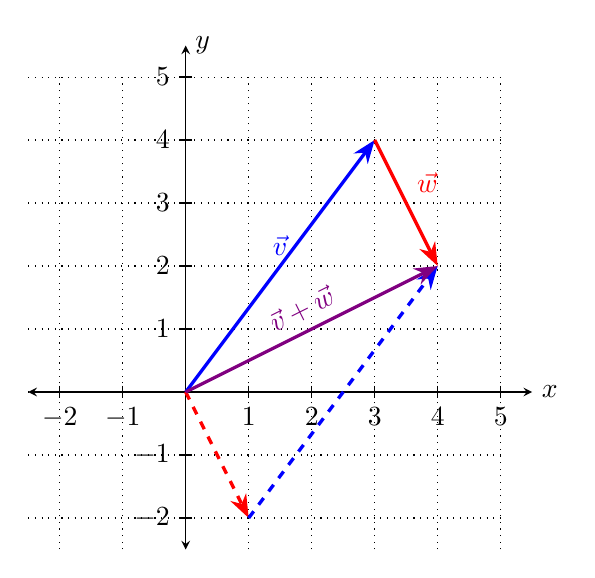
\begin{tikzpicture}[scale=0.8]
    \draw [dotted] (-2.5,-2.5) grid (5,5);
    \draw [<->,>=stealth] (-2.5,0) -- (5.5,0) node [right] {$x$};
    \draw [<->,>=stealth] (0,-2.5) -- (0,5.5) node [right] {$y$};
    \foreach \x in {-2,-1,,1,2,3,4,5}
    \draw (\x, 0.1) -- (\x,-0.1) node [below] {$\x$};
    \foreach \y in {-2,-1,,1,2,3,4,5}
    \draw (0.1,\y) -- (-0.1,\y) node [left] {$\y$};
    \draw [-{Stealth}, very thick, color=blue] (0,0) -- (3,4) node [midway, above] {$\vec{v}$};
    \draw [-{Stealth}, very thick, color=red] (3,4) -- +(1,-2) node [midway, above right] {$\vec{w}$};
    \draw [-{Stealth}, very thick, dashed, color=red] (0,0) -- (1,-2);
    \draw [-{Stealth}, very thick, color=blue, dashed] (1,-2) -- +(3,4);
    \draw [-{Stealth}, very thick, color=violet] (0,0) -- (4,2) node [midway, sloped, above] {$\vec{v}+\vec{w}$};
\end{tikzpicture}
\end{center}
\end{frame}

% \begin{frame}{Operation Properties of Vectors}
% The component form of vectors allows us to justify the following properties for $\vec{v}=\langle v_1, v_2 \rangle$ and $\vec{w}=\langle w_1, w_2 \rangle$: \newline\\
% \begin{itemize}
%     \onslide<2->{\item $\vec{v} + \vec{w} = \langle v_1 + w_1, v_2 + w_2 \rangle$}
%     \onslide<3->{\item $\vec{v} - \vec{w} = \langle v_1 - w_1, v_2 - w_2 \rangle$}
%     \onslide<4->{\item $\vec{v} + \vec{w} = \vec{w} + \vec{v}$ (Commutative Prop.)}
%     \onslide<5->{\item $(\vec{u} + \vec{v}) + \vec{w} = \vec{u} + (\vec{v} + \vec{w})$ (Associative Prop.)}
%     \onslide<6->{\item $\vec{v} + \vec{0} = \vec{v}$ (Identity Property)}
%     \onslide<7->{\item $\vec{v} + (-\vec{v}) = 0$ (Inverse Prop.)}
% \end{itemize}    
% \end{frame}

% \begin{frame}{Example 2}
%     Let $\vec{v} = \langle 3, 4 \rangle$ and suppose $w = \overrightarrow{PQ}$ where $P(-3, 7)$ and $Q(-2, 5)$. Find $\vec{v} + \vec{w}$ and interpret the result geometrically.
%     \begin{align*}
%         \onslide<2->{\vec{w} &= \langle -2-(-3), 5-7\rangle} \\[11pt]
%         \onslide<3->{&= \langle 1,-2\rangle} \\[11pt]
%         \onslide<4->{\vec{v}+\vec{w} &= \langle 3+1, 4-2\rangle} \\[11pt]
%         \onslide<5->{&=\langle 4, 2\rangle}
%     \end{align*}
% \end{frame}

% \begin{frame}{Example 2}
%     Geometrically, $\vec{v}+\vec{w}$ is as follows:
% \begin{center}
% \begin{tikzpicture}[scale=0.8]
%     \draw [dotted] (-2.5,-2.5) grid (5,5);
%     \draw [<->,>=stealth] (-2.5,0) -- (5.5,0) node [right] {$x$};
%     \draw [<->,>=stealth] (0,-2.5) -- (0,5.5) node [right] {$y$};
%     \foreach \x in {-2,-1,,1,2,3,4,5}
%     \draw (\x, 0.1) -- (\x,-0.1) node [below] {$\x$};
%     \foreach \y in {-2,-1,,1,2,3,4,5}
%     \draw (0.1,\y) -- (-0.1,\y) node [left] {$\y$};
%     \draw [-{Stealth}, very thick, color=blue] (0,0) -- (3,4) node [midway, above] {$\vec{v}$};
%     \draw [-{Stealth}, very thick, color=red] (3,4) -- +(1,-2) node [midway, above right] {$\vec{w}$};
%     \draw [-{Stealth}, very thick, dashed, color=red] (0,0) -- (1,-2);
%     \draw [-{Stealth}, very thick, color=blue, dashed] (1,-2) -- +(3,4);
%     \draw [-{Stealth}, very thick, color=violet] (0,0) -- (4,2) node [midway, sloped, above] {$\vec{v}+\vec{w}$};
% \end{tikzpicture}
% \end{center}
% \end{frame}

\begin{frame}{Scalar Multiplication}
If we multiply our vector by a real number (a \alert{scalar}), we get a new vector.    \newline\\

\begin{tikzpicture}
    \coordinate (A) at (0,0);
    \coordinate (B) at (2,1);
    \coordinate (C) at (3,0);
    \coordinate (D) at (1,-1);
    \draw [-{Stealth}] (A) -- (B);
    \onslide<2->{\draw [-{Stealth}] (C) -- (D)};
    \node at (1,0.5) [below right, yshift=0.15cm] {$\vec{v}$};
    \onslide<2->{\node at (2,-0.5) [below right, yshift = 0.15cm] {$-\vec{v}$}};
    \coordinate (E) at (5,0);
    \coordinate (F) at (9,2);
    \onslide<3->{\draw [-{Stealth}] (E) -- (F) node [midway, below right] {$2\vec{v}$}};
\end{tikzpicture}   \\[11pt]
\onslide<4->{Scalar multiplication ``distributes" the scalar to both horizontal and vertical component.}
\end{frame}

\begin{frame}{Vector Subtraction}
Vector subtraction $\vec{v} - \vec{w}$ can be thought of as $\vec{v} + (-\vec{w})$ and is illustrated below:   \newline\\
\begin{center}
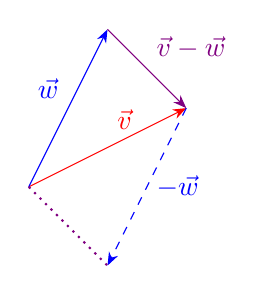
\begin{tikzpicture}
    \coordinate (A) at (0,0);
    \coordinate (B) at (2,1);
    \draw [-{Stealth}, color=red] (A) -- (B) node [midway, above right, yshift=0.1cm] {$\vec{v}$};
    \coordinate (C) at (1,2);
    \draw [-{Stealth}, color=blue] (A) -- (C) node [midway, above left] {$\vec{w}$};
    \coordinate (D) at (1,-1);
    \draw [-{Stealth}, color=blue, dashed] (B) -- (D) node [midway, right] {$-\vec{w}$};
    \draw [-{Stealth}, color=violet] (C) -- (B) node [midway, above right] {$\vec{v}-\vec{w}$};
    \draw [dotted, color=violet, thick] (A) -- (D);
\end{tikzpicture}    
\end{center}
\end{frame}

\begin{frame}{Example 2a}
If $\mathbf{v} = 5\mathbf{i} + 4\mathbf{j}$, and $\vec{w} = \langle 6,-9 \rangle$, find each of the following.  \newline\\

(a) \quad $\mathbf{v} + \mathbf{w}$
\begin{align*}
    \onslide<2->{\mathbf{v}+\mathbf{w} &= \langle 5,4\rangle + \langle 6,-9 \rangle} \\[8pt]
    \onslide<3->{&= \langle 5+6, 4+(-9)\rangle} \\[8pt]
    \onslide<4->{&= \langle 11, -5\rangle}  \\
\end{align*}
\end{frame}

\begin{frame}{Example 2b}
(b) \quad $\mathbf{v} - \mathbf{w}$ 
\begin{align*}
    \onslide<2->{\mathbf{v}-\mathbf{w} &= \langle 5, 4\rangle - \langle 6, -9\rangle} \\[8pt]
    \onslide<3->{&=\langle 5-6, 4-(-9)\rangle} \\[8pt]
    \onslide<4->{&=\langle -1, 13\rangle} \\
\end{align*}
\end{frame}

\begin{frame}{Example 2c}
(c) \quad $6\vec{v}$
\begin{align*}
    \onslide<2->{6\vec{v} &= 6\langle5, 4\rangle} \\[8pt]
    \onslide<3->{&= \langle 30, 24\rangle} \\
\end{align*}
\end{frame}

\begin{frame}{Example 2d}
(d) \quad $2\mathbf{v} + 4\mathbf{w}$
\begin{align*}
\onslide<2->{2\mathbf{v}+4\mathbf{w} &= 2(5\mathbf{i} + 4\mathbf{j}) + 4(6\mathbf{i}-9\mathbf{j})} \\[8pt]
\onslide<3->{&=10\mathbf{i}+8\mathbf{j} + 24\mathbf{i} - 36\mathbf{j}} \\[8pt]
\onslide<4->{&=34\mathbf{i} - 28\mathbf{j}} \\
\end{align*}
\end{frame}

% \begin{frame}{Scalar Properties}
% \begin{itemize}
%     \item $(kr)\vec{v} = k(r\vec{v})$ (Associative Prop.)
%     \onslide<2->{\item $1\vec{v} = \vec{v}$ (Identity Prop.)}
%     \onslide<3->{\item $-\vec{v} = -1\vec{v}$ (Additive Inverse Prop.)}
%     \onslide<4->{\item $(k + r)\vec{v} = k\vec{v} + r\vec{v}$ (Distributive Prop. over Scalar Addition)}
%     \onslide<5->{\item $k(\vec{v} + \vec{w}) = k\vec{v} + k\vec{w}$ (Distributive Prop. over Vector Addition)}
%     \onslide<6->{\item $k\vec{v} = 0 \text{ if and only if } k = 0 \text{ or } \vec{v} = 0$ (Zero Product Prop.)}
% \end{itemize}
% \end{frame}

% \begin{frame}{Example 3}
% Solve $5\vec{v} - 2(\vec{v} + \langle 1, -2\rangle ) = \vec{0}$ for $\vec{v}$.    
% \begin{align*}
%     \onslide<2->{5\vec{v} - 2(\vec{v} + \langle 1, -2\rangle ) &= \langle 0, 0 \rangle} \\[11pt]
%     \onslide<3->{5\langle x,y\rangle - 2\left(\langle x,y \rangle + \langle 1, -2 \rangle \right) &= \langle 0, 0 \rangle}    \\[11pt]
%     \onslide<4->{\langle 5x, 5y\rangle - 2\langle x+1, y-2\rangle &= \langle 0, 0 \rangle} \\[11pt]
%     \onslide<5->{\langle 5x, 5y \rangle - \langle 2x+2, 2y-4\rangle &= \langle 0, 0 \rangle} \\[11pt]
%     \onslide<6->{\langle 3x-2, 3y+4\rangle &= \langle 0, 0 \rangle} \\[11pt]
%     \onslide<7->{3x-2=0 \quad & 3y+4=0} \\[11pt]
%     \onslide<8->{x = \frac{2}{3} \quad & y = -\frac{4}{3} \longrightarrow \left< \frac{2}{3}, -\frac{4}{3} \right>}
% \end{align*}
% \end{frame}

\section{Finding Unit Vectors} 

\begin{frame}{Unit Vectors}
A \alert{unit vector}, $\hat{v}$, is a vector that has a magnitude of 1.   \newline\\

\begin{center}
\begin{tikzpicture}
    \draw (-2,0) -- (2,0) node [below right] {$x$};
    \draw (0,-2) -- (0,2) node [right] {$y$};
    \draw (-1,0.2) -- (-1,-0.2) node [below] {\tiny$-1$};
    \draw (1, 0.2) -- (1, -0.2) node [below] {\tiny$1$};
    \draw (0.2, 1) -- (-0.2,1) node [left] {\tiny$1$};
    \draw (0.2,-1) -- (-0.2,-1) node [left] {\tiny$-1$};
    \draw [dashed, color=red] (0,0) circle (1cm);
    \draw [->, >=stealth, color=blue] (0,0) -- (60:2) node [right] {$\vec{v}$};
    \draw [->, >=stealth, line width = 1.25] (0,0) -- (60:1) node [right] {$\hat{v}$};
\end{tikzpicture}
\end{center} 

Notice the unit vector $\hat{v}$ is parallel to $\vec{v}$.      \newline\\

$\mathbf{i}$ and $\mathbf{j}$ are unit vectors with $\mathbf{i}=\langle 1,0 \rangle$ and $\mathbf{j} = \langle 0, 1\rangle$
\end{frame}

\begin{frame}{Unit Vectors}
 We get $\hat{v}$ by dividing the magnitude of $\vec{v}$ by itself:
\[
\hat{v} = \dfrac{\vec{v}}{\lVert v \rVert}
\]
\\[11pt]
\pause 
Since we are dividing the vector (the hypotenuse) by the magnitude, we also divide the $x$ and $y$ components as well:
\[
    \hat{v} = \left \langle \dfrac{x}{\lVert v \rVert}, \dfrac{y}{\lVert v \rVert} \right \rangle
\]   
\end{frame}

\begin{frame}{Example 3a}
    Find a unit vector for each given vector.   \newline\\
(a) \quad $\mathbf{v} = 5\mathbf{i} - 12\mathbf{j}$
\begin{align*}
    \onslide<2->{\lVert \mathbf{v} \rVert &= \sqrt{5^2 + 12^2}} \\[8pt]
    \onslide<3->{&= 13} \\[8pt]
    \onslide<4->{\hat{v} &= \frac{5}{13}\mathbf{i} - \frac{12}{13}\mathbf{j}} \\
\end{align*}
\end{frame}

\begin{frame}{Example 3b}
(b) \quad $\vec{w} = \langle 4, -3 \rangle$
\begin{align*}
    \onslide<2->{|\vec{w}| &= \sqrt{4^2 + 3^2}} \\[8pt]
    \onslide<3->{&= 5} \\[8pt]
    \onslide<4->{\hat{w} &= \left< \frac{4}{5}, -\frac{3}{5}\right>} \\
\end{align*}
\end{frame}

\begin{frame}{Example 3c}
(c) \quad $\mathbf{d} = 7\mathbf{i} + \mathbf{j}$
\begin{align*}
\onslide<2->{|\mathbf{d}| &= \sqrt{7^2 + 1^2}} \\[8pt]
\onslide<3->{&= \sqrt{50}} \\[8pt]
\onslide<4->{&=5\sqrt{2}} \\[8pt]
\onslide<5->{\hat{d} &= \frac{7}{5\sqrt{2}}\mathbf{i} + \frac{1}{5\sqrt{2}}\mathbf{j}} \\[11pt]
\onslide<6->{&= \frac{7\sqrt{2}}{10}\mathbf{i} + \frac{\sqrt{2}}{2}\mathbf{j}} \\
\end{align*}
\end{frame}

\section{Find Component Form from Magnitude and Direction and Vice Versa}

\begin{frame}{Magnitude and Direction}
If we place a vector $\langle x, y \rangle$ in the coordinate plane, we can put the initial point at the origin and the terminal point at $(x, y)$.  \newline\\
\begin{center}
\begin{tikzpicture}
    \draw [<->, >=stealth] (-2, 0) -- (2, 0) node [right] {$x$};
    \draw [<->, >=stealth] (0, -2) -- (0, 2) node [right] {$y$};
    \draw [-{stealth}] (0,0) -- (1,1.5);
    \draw [fill=black] (1,1.5) circle (1pt);
    \draw [dashed] (1,1.5) -- (1,0);
    \node at (0,0) [above right, xshift = 0.1cm] {\small$\theta$};
    \node at (1,1) [left,xshift=-0.25cm] {$\lVert \vec{v} \rVert$};
    \node at (0.5,0) [below] {$x$};
    \node at (1,0.75) [right] {$y$};
    \node at (1,1.5) [right] {$(x, y)$};
\end{tikzpicture}    
\end{center}
\end{frame}

\begin{frame}{Magnitude and Direction}
    From Trig Functions of Any Angle, \[x = \lVert \vec{v} \rVert \cos \theta \text{ and } y = \lVert \vec{v} \rVert \sin \theta\]. 
\pause 
Thus, \[\langle x, y \rangle = \langle \lVert \vec{v} \lVert \cos\theta, \lVert \vec{v} \rVert \sin \theta  \rangle = \lVert \vec{v} \rVert \langle \cos \theta, \sin \theta \rangle\]
\end{frame}

\begin{frame}{Example 4}
Find the horizontal and vertical component form of the vector whose magnitude and direction angle are given by $|u|=12$ and $\theta=150^\circ$.
\begin{align*}
\onslide<2->{x = 12\cos150^\circ \quad & \quad y = 12\sin150^\circ} \\[8pt]
\onslide<3->{x = 12\left(-\frac{\sqrt{3}}{2}\right) \quad & \quad y = 12\left(\frac{1}{2}\right)} \\[8pt]
\onslide<4->{x = -6\sqrt{3} \quad & \quad y = 6} \\[8pt]
\onslide<5->{\langle -6\sqrt{3}, &\quad 6\rangle} \\
\end{align*}
% Find the component form of the vector with $\lVert \vec{v} \rVert = 5$, with $\vec{v}$ in Quadrant II and makes a $60^\circ$ angle with the negative $x$-axis. \newline\\  
% \pause
% If the angle makes a $60^\circ$ with the negative $x$-axis in quadrant II, then the total amount rotated must be $180^\circ - 60^\circ = 120^\circ$.
% \begin{minipage}{0.4\textwidth}
% \begin{tikzpicture}
% \draw [<->, >=stealth] (-2,0) -- (2,0);
% \draw [<->, >=stealth] (0,-2) -- (0,2);
% \draw [-{Stealth}, thick, color=blue] (0,0) -- (120:2);
% \draw [->, >=stealth, color=red] (0.75,0) arc (0:120:0.75) node [midway, above] {$120^\circ$};
% \draw [color=blue] (120:0.5) arc (120:180:0.5) node [midway, left] {$60^\circ$};
% \end{tikzpicture}
% \end{minipage}
% \begin{minipage}{0.4\textwidth}
% \begin{align*}
%     \onslide<3->{\vec{v} &= 5\langle \cos 120^\circ, \sin 120^\circ \rangle} \\[11pt]
%     \onslide<4->{&= 5\left< -\frac{1}{2}, \frac{\sqrt{3}}{2}\right>} \\[11pt]
%     \onslide<5->{&= \left<-\frac{5}{2}, \frac{5\sqrt{3}}{2}\right>}
% \end{align*}
% \end{minipage}
\end{frame}

\begin{frame}{Example 5}
For $\vec{v} = \langle 3, -3\sqrt{3} \rangle$, find $\lVert \vec{v} \rVert$ and $\theta$ ($0 \leq \theta < 2\pi$) and write in $\lVert \vec{v} \rVert \langle \cos \theta, \sin \theta \rangle$ form. 
\begin{align*}
    \onslide<2->{\lVert \vec{v} \rVert &= \sqrt{3^2+(3\sqrt{3})^2}} \\[11pt]
    \onslide<3->{&= \sqrt{36} = 6}  \\
\end{align*}
\end{frame}
\begin{frame}{Example 5}
For $\vec{v} = \langle 3, -3\sqrt{3} \rangle$, find $\lVert \vec{v} \rVert$ and $\theta$ ($0 \leq \theta < 2\pi$) and write in $\lVert \vec{v} \rVert \langle \cos \theta, \sin \theta \rangle$ form.
\begin{align*}
    \onslide<1->{\theta' &= \tan^{-1}\left|\frac{-3\sqrt{3}}{3}\right|} \\[11pt]
    \onslide<2->{\theta ' &= 60^\circ} \\[11pt]
    \onslide<3->{\theta &= 360^\circ - 60^\circ = 300^\circ} \\[8pt]
    \onslide<4->{&= \frac{5\pi}{3}}
\end{align*}
\begin{center}
\onslide<5->{$6\left< \cos\left(\frac{5\pi}{3}\right), \sin\left(\frac{5\pi}{3}\right)\right>$}
\end{center}
\end{frame}

% \begin{frame}{Example 6a}
% Given $\vec{v} = \langle 3, 4 \rangle$ and $\vec{w} = \langle 1, -2 \rangle$, find each of the following.  \newline\\
% (a) \quad $\hat{v}$
% \begin{align*}
%     \onslide<2->{|\vec{v}| &= \sqrt{3^2+4^2}} \\
%     \onslide<3->{&= 5} \\
%     \onslide<4->{\hat{v} &= \left< \frac{3}{5}, \frac{4}{5} \right>}
% \end{align*}
% \end{frame}

% \begin{frame}{Example 6b}
% (b) \quad $\lVert \vec{v} \rVert - 2 \lVert \vec{w} \rVert$
% \begin{align*}
%     \onslide<2->{\lVert \vec{v} \rVert &= 5} \\
%     \onslide<3->{\lVert \vec{w} \rVert &= \sqrt{1^2+2^2} = \sqrt{5}} \\
%     \onslide<4->{\lVert \vec{v} \rVert - 2 \lVert \vec{w} \rVert &= 5 - 2\sqrt{5}}
% \end{align*}
% \end{frame}

% \begin{frame}{Example 6c}
% (c) \quad $\lVert \vec{v} - 2\vec{w}\rVert$
% \begin{align*}
%     \onslide<2->{\lVert \vec{v} - 2\vec{w} \rVert &= \lVert \langle 3, 4\rangle - 2\langle 1, -2 \rangle \rVert} \\[8pt]
%     \onslide<3->{&= \lVert \langle 3, 4\rangle - \langle 2,-4 \rangle \rVert} \\[8pt]
%     \onslide<4->{&= \lVert \langle 1, 8\rangle \rVert} \\[8pt]
%     \onslide<5->{&= \sqrt{1^2 + 8^2} = \sqrt{65}}
% \end{align*}
% \end{frame}

% \begin{frame}{Example 6d}
% (d) \quad $\lVert \hat{w} \rVert$
% \begin{align*}
%     \onslide<2->{\lVert \hat{w} \rVert &= 1 \text{ \quad (magnitude of any unit vector is 1)}}
% \end{align*}
% \end{frame}

\end{document}
